\documentclass{standalone}

\RequirePackage[T1]{fontenc} \RequirePackage[tt=false, type1=true]{libertine}
\RequirePackage[varqu]{zi4} \RequirePackage[libertine]{newtxmath}

\pdfoutput=1

\usepackage{amsfonts}
\usepackage{tikz}
\usetikzlibrary{arrows.meta}

\begin{document}


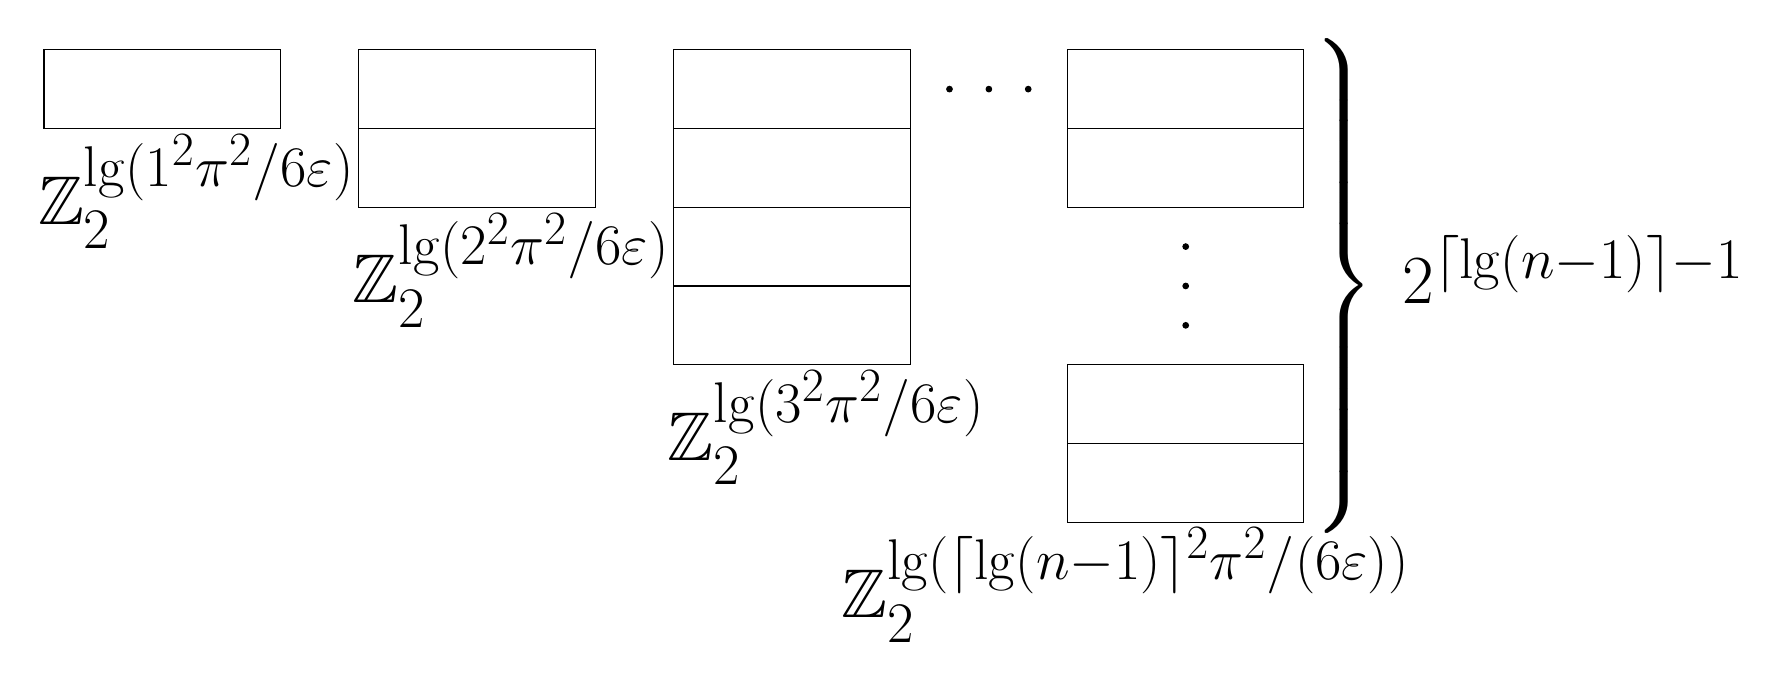
\begin{tikzpicture}

\draw (0,0) rectangle (3,1);
\draw (-0.2,-0.8) node[right] {\Huge $\mathbb{Z}_2^{\lg (1^2 \pi^2 /6 \varepsilon)}$};

\draw (4,0) rectangle (7,1);
\draw (4,0) rectangle (7,-1);
\draw (3.8,-1.8) node[right] {\Huge $\mathbb{Z}_2^{\lg (2^2 \pi^2 /6 \varepsilon)}$};

\draw (8,1) rectangle (11,-3);
\draw (8,0) rectangle (11,-2);
\draw (8,-1) -- (11,-1);
\draw (7.8,-3.8) node[right] {\Huge $\mathbb{Z}_2^{\lg (3^2 \pi^2 /6 \varepsilon)}$};

\filldraw (11.5,0.5) circle (1pt);
\filldraw (12,0.5) circle (1pt);
\filldraw (12.5,0.5) circle (1pt);

\draw (13,1) rectangle (16,-1);
\draw (13,0) -- (16,0);
\filldraw (14.5,-1.5) circle (1pt);
\filldraw (14.5,-2) circle (1pt);
\filldraw (14.5,-2.5) circle (1pt);
\draw (13,-3) rectangle (16,-5);
\draw (13,-4) -- (16,-4);

\draw (10,-5.8) node[right] {\Huge$\mathbb{Z}_2^{\lg (\lceil\lg (n-1)\rceil^2 \pi^2 /(6 \varepsilon))}$};

\draw (16,-2) node[right]{\Huge$\left\}\begin{array}{c} \\ \\ \\ \\ \\ \\ \end{array}2^{\lceil \lg (n-1)\rceil-1}\right.$};


%% \draw (1,0) node[right] {$\mathbb{Z}_2^{\lceil \lg n \rceil + \lg (1/\varepsilon) + 2}$};
%% \draw (4,0) node[right] {$\mathbb{Z}_2^0$ or $\mathbb{Z}_2^1$ or \ldots or $\mathbb{Z}_2^{\lg \lg U}$};

%% \draw (0,0.4) rectangle (6,1);
%% \draw (4,0.4) -- (4,1);

%% \filldraw (4,1.3) circle (1pt);
%% \filldraw (4,1.6) circle (1pt);
%% \filldraw (4,1.9) circle (1pt);

%% \draw (0,2.2) rectangle (6,4);
%% \draw (0,2.8) rectangle (6,3.4);
%% \draw (4,2.2) -- (4,4);


\end{tikzpicture}

\end{document}
